This section should describe the overall structure of your software system. Think of it as the strategy for how you will build the system. An architectural "layer" is the top-level logical view, or an abstraction, of your design. Layers should be composed of related elements of similar capabilities, and should be highly independent of other layers, but should have very clearly defined interfaces and interactions with other layers. Each layer should be identified individually and should be unique as to its function and purpose within the system. This section should also contain the high-level block diagram of the layers, as shown in the example below, as well as detailed descriptions of the functions of each layer.

\begin{figure}[h!]
	\centering
 	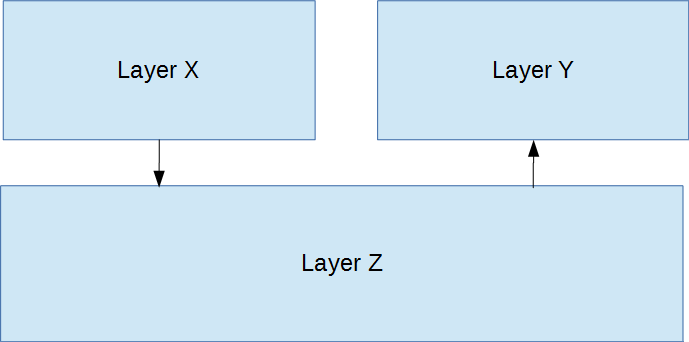
\includegraphics[width=0.60\textwidth]{images/layers}
 \caption{A simple architectural layer diagram}
\end{figure}

\subsection{Computer Vision Layer}
This layer is the heart of the core autonomous functionalities of the Turing Board. We use computer vision and depth imagery to determine the board's surroundings and calculate the best path to move forward. The user will have, strapped around their ankle, an elastic band affixed with a pattern of ArUco markers for the \textit{Follow Along} feature. This layer tracks the movement of the user vis-a-vis the anklet to determine how to instruct the combination of motors to move so as to follow the user at an appropriate pace. It is also responsible for detecting possible obstacles when operating on its own to find the user as part of the \textit{Summon} feature. 
Data taken in from the cameras will flow from this layer into the Main Control Layer to be processed and then send out the appropriate signals primarily to the Wheels \& Turning Layer. This layer also takes in data from the anklet component in the HMI layer specifically for the Follow feature.

\subsection{Remote Control Layer}
This layer is controlled directly by the user. It takes the form of an app that sends data to the Main Control layer for the appropriate signals to be sent to the other layers. The app requires an authentication process to log into it. It will also provide the user with ride data analysis after a trip on the board is completed. This app is available on iOS and Android.

\subsection{Power Layer}
This layer is responsible for controlling the power distributed to the electrical components on the Turing Board. It directly powers portions of both the HMI layer and the Wheels \& Turning layer. This layer ensures power is not over-distributed by way of a Buck converter. It also provides data on how much charge is left in the battery at any given time. This data is sent to the Main Controls layer for the appropriate signals to be sent out to the other layers as needed.

\subsection{Main Controls Layer}
This layer is in charge of processing and sending out the majority of the signals on the Turning Board. It receives data from the Computer Vision layer, the Remote Control Layer, and the Power layer. With these inputs, it sends data to the HMI layer as well as the Wheels \& Turning layer. The Jetson TX2 provides the computing power in this layer and will process all of these needs. It will also fetch data from a real-time database and directly interact with a separate micro-controller that is in charge of the minor systems on the Turing Board.

\subsection{HMI Layer}
This layer contains all of the hardware parts of the Turing Board that interacts directly with the user. This layer includes LEDs, a pressure sensor, a buzzer/speaker, and an anklet. The LEDs let the user know what mode the board is in (Summon, Follow, or Electric) based off of the color they are emitting at the time. The pressure sensor determines how much weight is currently on the board and transmits this information to the Main Controls layer to control what mode the board is in. The buzzer or speaker will make a sound if the user steps onto the board when it is not in Electric mode to notify them of improper usage. Finally, the anklet is to be worn by the user to give data to the Computer Vision layer when the board is in Follow mode.

\subsection{Wheels \& Turning Layer}
This layer contains the components needed to cause the board to move and turn. It contains the ESC, brushless motors, stepper motors, optical sensors for the stepper motors, solenoids, optical sensors for the solenoids, the micro-controller, and the turning mechanism. The ESC will control the speed at which the brushless motors inside of the wheels turn as determined by signals sent from the Main Controls layer. The stepper motor will turn the turning mechanism a certain amount of degrees not exceeding 30-45 in either direction as determined by the Main Controls layer. The optical sensor for the stepper motor will track how many degrees the turning mechanism has been turned and send this data to the Main Controls layer. The solenoids will be responsible for locking the turning mechanism in place when it is in Electric mode. The optical sensors for the solenoids will determine if the solenoids are properly locked in place or not and transmit this data to the Main Controls layer. The micro-controller will receive data from the Main Controls layer and use that to output the necessary signals to the motors. 

